\RequirePackage{fix-cm,cmap}
\documentclass[
fontsize=11pt,
paper=a4,
abstract=true,
numbers=noenddot,
listof=totoc,
bibliography=totoc,
twoside,
open=right,
cleardoublepage=plain,
parskip=half+, % comment this out if you do not want an empty half line between paragraphs, but please read the KomaScript Guide and search for parskip (around page 82): ftp://ftp.dante.de/pub/tex/macros/latex/contrib/koma-script/scrguide.pdf
BCOR=1cm, % Bindekorrektur: Change this accordingly, also read the KomaScript Guide! Make sure you read the guide.
]{scrreprt}

%\documentclass[a4paper,10pt]{article}
\usepackage[utf8]{inputenc}
\usepackage[english]{babel}
\usepackage{geometry}
\usepackage[T1]{fontenc}
\usepackage{float}
\usepackage{multirow}
\usepackage{booktabs}
\usepackage{chemfig}
\usepackage{amsmath}
\usepackage{xcolor}
\usepackage{pxfonts}
\usepackage{tikz}
\usepackage{hyperref}
\usepackage{listings}
\usepackage{multido}

\definecolor{commentgreen}{RGB}{2,112,10}
\definecolor{eminence}{RGB}{108,48,130}
\definecolor{weborange}{RGB}{255,165,0}
\definecolor{frenchplum}{RGB}{129,20,83}



% Environment for Xtext code
\lstdefinelanguage{Xtext}
{
    morekeywords={grammar, with, hidden, generate, as, import, returns, current, terminal, enum},
    morecomment=[l]{//},
    morecomment=[s]{/*}{*/},
    morestring=[b]",
    tabsize=4,
    commentstyle=\color{commentgreen},
    keywordstyle=\color{eminence},
    stringstyle=\color{red}
}


\title{Domain-Specific Languages with Xtext or Scala: Final report}
\author{Dominik Habermann (108019250645)\\Masuthan Mathiyalakan (108017235408)}



\newcommand{\gerquot}[1]{\glqq#1\grqq}
\newcommand{\dashAndSpace}{\textendash \space}
\newcommand{\dashAndSpaceSeq}[1]{\dashAndSpace#1 \textendash}

\newcommand{\DSL}{domain specific language}
\newcommand{\CFG}{context-free grammar}
\newcommand{\IUPAC}{International Union of Pure and Applied Chemistry}
\newcommand{\ENBF}{Extended Backus-Naur Form}

\newcommand{\captionVSpace}{\vspace*{-0.05cm}}
\newcommand{\connectionThicknessDefault}{1.5pt}
\newcommand{\CFGDefinitionSize}{0.60}
\newcommand{\SymbolDescriptionTable}{0.35}
\newcommand{\screenshotWidth}{1.0}

\newcommand{\colorBracketFirstNesting}{black}
\newcommand{\colorBracketSecondNesting}{blue}
\newcommand{\colorBracketThirdNesting}{green}
\newcommand{\colorBracketFourthNesting}{red}
\newcommand{\colorBracketFifthNesting}{cyan}
\newcommand{\colorBracketSixthNesting}{yellow}
\newcommand{\colorBracketSeventhNesting}{brown}
\newcommand{\colorBracketEigthNesting}{orange}

\newcommand{\colorNew}{orange}
\newcommand{\colorMainChain}{blue}
\newcommand{\colorBranchFirstNesting}{orange}
\newcommand{\colorBranchSecondNesting}{cyan}

% Replacements for specific words, that can be written in multiple ways
\newcommand{\nonterminal}{non terminal}
\newcommand{\metamodel}{meta model}

%%%%% %%%%% %%%%% %%%%% %%%%% %%%%% %%%%% %%%%%                %%%%% %%%%% %%%%% %%%%% %%%%% %%%%% %%%%% %%%%%
%%%%% %%%%% %%%%% %%%%% %%%%% %%%%% %%%%% %%%%% BEGIN document %%%%% %%%%% %%%%% %%%%% %%%%% %%%%% %%%%% %%%%%
%%%%% %%%%% %%%%% %%%%% %%%%% %%%%% %%%%% %%%%%                %%%%% %%%%% %%%%% %%%%% %%%%% %%%%% %%%%% %%%%%
\begin{document}

% \input{frontpage}

\pagenumbering{arabic} %switches to arabic numbers for the rest of the text
\setcounter{page}{1}

\maketitle
\tableofcontents

\chapter{Introduction}\label{s:Introduction}
%To understand technologies like DSLs (\DSL) examples are the %best way to explain different aspects, e.g. use cases, %typical problems, limitations, etc. Instead of creating an %artificial example, in general a real world instance offers a %more plain view to a technology.
Technologies like DSLs (\DSL) can be understood with examples, which serve as best way to explain different aspects, e.g. use cases, typical problems, limitations, etc. They can be even better understood, when instead of an artificial example, a real world example is created, which offers a more plain view to a technology.

Because of this reason the IUPAC naming system as an example was chosen. This is a naming convention from the chemistry, especially in the organic chemistry this convention is used frequently. For classification: \emph{This report focuses on the naming system itself} and has only low contact points to the chemical background.

This document is the final report of the Project 18: \emph{Domain-Specific Languages with Xtext or Scala} in WS 23/24. The chapter \ref{s:IntroductionToTheIUPACNomenclature} (\nameref{s:IntroductionToTheIUPACNomenclature}) contains historical background and an introduction to the domain on an abstract level. Basic rules are introduced and corresponding to the new rule a possible \CFG \space is proposed. In the chapter \ref{s:Xtext} the implementation via Xtext is shown; at the begin the abstract syntax via a meta model and suitable Xtext code as an implementation of the concrete syntax. At the end a discussion with conclusion as well as a reflection is given in the last two chapters \ref{s:DiscussionandConclusion} + \ref{s:Reflection}.

% The goal is to make a tutorial, that explains the creation of CFG (\CFG) and illustrate the differences of abstract syntax and concrete syntax. We do not expect, that you are a expert in this topic; but a basic knowledge should be available. Terms like \gerquot{grammar} or \gerquot{production rule} will not be explained.



\chapter{Introduction to the IUPAC nomenclature}\label{s:IntroductionToTheIUPACNomenclature}
\section{History of the IUPAC naming convention}\label{ss:HistoryOfTheIUPACNamingConvention}
IUPAC is an abbreviation for \emph{\IUPAC}. This union was founded in 1919 with the goal to simplify the global communication between chemists. Up to this year no global rules were available for naming chemical structures. Every country used his own system and this leaded to many misunderstandings; sometimes even in a single country. The situation can be compared like before the metric system was introduced.

The IUPAC invented a systematic way to create a unique\footnote{A unique name is only with the implementation of all semantic rules possible.} name for \dashAndSpaceSeq{in theory} every chemical structure. In most cases the literature uses the term \gerquot{IUPAC name} or \gerquot{IUPAC nomenclature} for a name in the IUPAC convention. In this report both of this terms will be also used.

The rules of this naming convention can be formulated as \CFG. So it can be also understood as a kind of DSL. In the following sections basic rules of the naming convention will be introduced. And also the way to cast it to a \CFG.

Carbon (C) has the unique skill to create long structures with branches and nesting, that are stable \dashAndSpace in a chemical point of view. The possibilities are tremendous. Almost all other elements are not capable of creating larger structures. So the naming convention focuses on the carbon and the describing of that structures.



\section{Nothing than straight chains}\label{ss:NothingThanStraightChains}
In a simplified manner carbon atoms can be compared with building blocks: The simplest way is a straight chain of carbon atoms without any branches. The IUPAC nomenclature encodes the length of such a straight chain in specific terms like \gerquot{Methan}, \gerquot{Ethan}, etc. See the table \ref{tab:NumCarbonEncodedName} below for a length up to 10 carbon atoms.

\begin{table}[H]
    \centering
    \begin{tabular}{c|l}
        \toprule
        \textbf{Number of carbon atoms} & \textbf{Encoded name} \\
        \midrule
        1 & Methan \\
        2 & Ethan \\
        3 & Propan \\
        4 & Butan \\
        5 & Pentan \\
        6 & Hexan \\
        7 & Heptan \\
        8 & Octan \\
        9 & Nonan \\
        10 & Decan \\
        \bottomrule
    \end{tabular}
    \captionVSpace
    \caption{List of the first 10 names for a straight chain}
    \label{tab:NumCarbonEncodedName}
\end{table}

\noindent For example: \\
\emph{Ethan}\qquad
\setchemfig{chemfig style={line width=\connectionThicknessDefault}}
\chemfig{C-C} \\
or \\
\emph{Hexan}\qquad
\setchemfig{chemfig style={line width=\connectionThicknessDefault}}
\chemfig{C-C-C-C-C-C} \\

In a sense of a grammar: This term for the straight chain is the main symbol. We call this symbol $c$ (for chain). $S$ is our mandatory start symbol and thus it is a \nonterminal\space symbol. For this tutorial $T$ the set for terminal symbols; $N$ for \nonterminal\space and $P$ for all production rules are used. In summary our first CFG grammar has the following definition:

\begin{figure}[H]
    \begin{minipage}[l]{\CFGDefinitionSize\textwidth}
        $$
        \begin{aligned}
            T &=& \{c\} \\
            N &=& \{S\} \\
            P &:& \\
            S &\rightarrow& c \\
        \end{aligned}
        $$
        \caption{The CFG with only straight chains.}
        \label{fig:CFGOnlyStraightChains}
    \end{minipage}
    \begin{minipage}[r]{\SymbolDescriptionTable\textwidth}
        \begin{table}[H]
        \centering
            \begin{tabular}{c|l}
                \toprule
                \textbf{Symbol} & \textbf{Description} \\
                \midrule
                c & Main chain \\
                \bottomrule
            \end{tabular}
            %\captionVSpace
            %\caption{Descriptions of the terminal symbols}
        \end{table}
    \end{minipage}
\end{figure}



\section{First order branches}\label{ss:FirstOrderBranches}
A chain of carbon atoms can also contain branches. This branches could also be nested; for now we focus on branches without deeper nesting. To identify a branch we need the length of this branch and the position. The position will be formulated from the point of view of the main chain. The length of the branch will be encoded in terms. These terms are comparable with the terms for the main chain but with a postfix \gerquot{yl} instead of \gerquot{an}. This are the first 4 terms for the encoded branch length:

\begin{table}[H]
    \centering
    \begin{tabular}{c|l}
        \toprule
        \textbf{Number of carbon atoms in branch} & \textbf{Encoded name} \\
        \midrule
        1 & Methyl \\
        2 & Ethyl \\
        3 & Propyl \\
        4 & Butyl \\
        \bottomrule
    \end{tabular}
    \captionVSpace
    \caption{List of the first 4 names for a branch}
    \label{tab:NumCarbonBranchEncodedName}
\end{table}

\noindent An example for this: \\
\begin{figure}[H]
    \centering
    \setchemfig{chemfig style={line width=\connectionThicknessDefault}}
    \chemfig{C-[,,,,\colorMainChain]C(-[6,,,,\colorBranchFirstNesting]C)-[,,,,\colorMainChain]C-[,,,,\colorMainChain]C-[,,,,\colorMainChain]C-[,,,,\colorMainChain]C-[,,,,\colorMainChain]C} \\
    \caption{Example with one branch of the length 1}
    \label{fig:SecondExample}
\end{figure}
The orange one is the branch with the length of one C atom. So the name is \emph{Methyl}. Any position information is written in front of the corresponding branch with a minus char between them. The full branch is therefore: \emph{2-Methyl}. The main chain has the length 7 $\rightarrow$ \emph{Heptan}.

So we can see, that a branch with the position information consists of three parts:
\begin{itemize}
    \item Position $p \in \mathbb{N}$
    \item Minus sign $m$
    \item Term for the length of the branch $b$
\end{itemize}
Because every branch has this structure, we can introduce a \nonterminal symbol to summarize all three terminals in this symbol $B$.

What about the order of branches and main chain? The IUPAC convention defines, that the term for the main chain will be always at the end of the name. This is good for the CFG definition, because we don't need to add production rules for both orders. With this and the other new information we have now following grammar (new elements are highlighted):

\begin{figure}[H]
    \begin{minipage}[l]{\CFGDefinitionSize\textwidth}
        $$
        \begin{aligned}
            T &=& \{c, {\color{\colorNew}p, m, b}\} \\
            N &=& \{S, {\color{\colorNew}B, M}\} \\
            P &:& \\
            S &\rightarrow& {\color{\colorNew}M} \\
            {\color{\colorNew}M} &\rightarrow& {\color{\colorNew}Bc} \\
            {\color{\colorNew}M} &\rightarrow& {\color{\colorNew}c} \\
            {\color{\colorNew}{B}} &\rightarrow& {\color{\colorNew}pmb} \\
        \end{aligned}
        $$
        \caption{CFG with exact one branch. $B \rightarrow pmb$ is an optional production rule.}
        \label{fig:CFGWithExactOneBranch}
    \end{minipage}
    \begin{minipage}[r]{\SymbolDescriptionTable\textwidth}
        \begin{table}[H]
        \centering
            \begin{tabular}{c|l}
                \toprule
                \textbf{Symbol} & \textbf{Description} \\
                \midrule
                c & Main chain \\
                p & position \\
                m & minus char \\
                b & branch \\
                \bottomrule
            \end{tabular}
            %\captionVSpace
            %\caption{Descriptions of the terminal symbols}
        \end{table}
    \end{minipage}
\end{figure}

It is important to notice, that an additional \nonterminal\space ($M$) was added. Because a grammar can only contains exact one start variable, we need $M$ as \gerquot{middle variable} to make words with and without branches possible. In summary: the $B$ is \dashAndSpaceSeq{like a branch} an optional \nonterminal.
The whole name of the structure in figure \ref{fig:SecondExample} is: \emph{2-MethylHeptan}\footnote{It can produced with
$
S
{\color{\colorBracketFirstNesting}{(}}
    M
    {\color{\colorBracketSecondNesting}{(}}
        B
        {\color{\colorBracketThirdNesting}{(}}
            pmb
        {\color{\colorBracketThirdNesting}{)}}
        , c
    {\color{\colorBracketSecondNesting}{)}}
{\color{\colorBracketFirstNesting}{)}}
$}.



\section{Multiple first order branches}\label{ss:MultipleFirstOrderBranches}
No one can forbid carbon atoms to create multiple branches of the same length. Let add an another branch of the length one at the third position:
\begin{figure}[H]
    \centering
    \setchemfig{chemfig style={line width=\connectionThicknessDefault}}
    \chemfig{C-[,,,,\colorMainChain]C(-[6,,,,\colorBranchFirstNesting]C)-[,,,,\colorMainChain]C(-[6,,,,\colorBranchFirstNesting]C)-[,,,,\colorMainChain]C-[,,,,\colorMainChain]C-[,,,,\colorMainChain]C-[,,,,\colorMainChain]C} \\
    \caption{Example with two branches of the length 1}
    \label{fig:ThirdExample}
\end{figure}

The intuitive way is to assume, that a second branch with the new position will be added to the begin of the name. It would be understandable; but it increases the name and in many molecules 5 branches and sometimes more are usual. For this reason there is a prefix to summarize branches of the same length. Table \ref{tab:BranchesWithTheSameLength} shows the first 4 prefixes.

\begin{table}[H]
    \centering
    \begin{tabular}{c|l}
        \toprule
        \textbf{Branches with the same length} & \textbf{Prefix} \\
        \midrule
        1 & Mono \\
        2 & Di \\
        3 & Tri \\
        4 & Tetra \\
        \bottomrule
    \end{tabular}
    \captionVSpace
    \caption{List of the first 4 prefixes to summarize branches with the same length}
    \label{tab:BranchesWithTheSameLength}
\end{table}

In normal cases the prefix \gerquot{Mono} is not used. So in the name \emph{1-MethylHeptan} is no \gerquot{Mono} missing! \textbf{The nomenclature defines no specific rules for the usage. For the introduction \gerquot{Mono} will be \underline{not used}. In the implementation \gerquot{Mono} will for the sake of simplicity be \underline{always used}.}\\

To identify also the second branch, we need the position of them. All position information will be written before the branch term and the prefix to summarize branches with the same length before the corresponding branch term: \emph{2,3-DiMethylHeptan}. Usually the positions are sorted in ascending order \dashAndSpace this is one possible static semantic rule. Between two numbers a comma is added to avoid ambiguous meanings if the positions larger than 9.

To formulate this in a grammar we have the situation, that position numbers can occur multiple times on the same branch term. So at least one production rule for branches needs to create a \nonterminal\space symbol. We can isolate the parts for the position information from the symbol $B \rightarrow pmb$ in a new symbol $C$. $p$ and $m$ will be moved to $C$, so that $C$ is now $C \rightarrow pm$. A second $C$, that creates itself, is necessary for multiple position information. This second $C$ could be: $C \rightarrow poC$ ($o$ represents here the comma char). \emph{Or in more simple words: we need to define production rules, they can create itself to make loops possible.}

With the prefix, that summarizes multiple branches (we call it $d$), we have a similar situation like with $M$. This prefix $d$ is an optional symbol, so we need an additional production rule to achieve this. An additional $B$ seems to be a good choice.

\begin{figure}[H]
    \begin{minipage}[l]{\CFGDefinitionSize\textwidth}
        $$
        \begin{aligned}
            T &=& \{c, p, m, b, {\color{\colorNew}o, d}\} \\
            N &=& \{S, B, M, {\color{\colorNew}C}\} \\
            P &:& \\
            S &\rightarrow& M \\
            M &\rightarrow& Bc \\
            M &\rightarrow& c \\
            % {\color{\colorNew}M} &\rightarrow& {\color{\colorNew}C} \\
            {\color{\colorNew}B} &\rightarrow& {\color{\colorNew}C} \\
            {\color{\colorNew}C} &\rightarrow& {\color{\colorNew}pmb} \\
            {\color{\colorNew}C} &\rightarrow& {\color{\colorNew}poC} \\
            {\color{\colorNew}C} &\rightarrow& {\color{\colorNew}mdb} \\
        \end{aligned}
        $$
        \caption{CFG with multiple branches and same length. Several usage of $C \rightarrow poC$ creates successive positions.}
        \label{fig:CFGWithMultipleBranchesAtTheSameLength}
    \end{minipage}
    \begin{minipage}[r]{\SymbolDescriptionTable\textwidth}
        \begin{table}[H]
        \centering
            \begin{tabular}{c|l}
                \toprule
                \textbf{Symbol} & \textbf{Description} \\
                \midrule
                c & Main chain \\
                p & position \\
                m & minus char \\
                b & branch \\
                o & comma char \\
                d & summary prefix \\
                \bottomrule
            \end{tabular}
            %\captionVSpace
            %\caption{Descriptions of the terminal symbols}
        \end{table}
    \end{minipage}
\end{figure}

\noindent The word \emph{2,3-DiMethylHeptan} can be produced with:
$
S
{\color{\colorBracketFirstNesting}{(}}
    M
    {\color{\colorBracketSecondNesting}{(}}
        C
        {\color{\colorBracketThirdNesting}{(}}
            po,
            C
            {\color{\colorBracketFourthNesting}{(}}
                po,
                C
                {\color{\colorBracketFifthNesting}{(}}
                    mdb
                {\color{\colorBracketFifthNesting}{)}}
            {\color{\colorBracketFourthNesting}{)}}
        {\color{\colorBracketThirdNesting}{)}}
        , c
    {\color{\colorBracketSecondNesting}{)}}
{\color{\colorBracketFirstNesting}{)}}
$\\


In theory we have the grammar, which fulfills the requirements. But with the production
$
S
{\color{\colorBracketFirstNesting}{(}}
    M
    {\color{\colorBracketSecondNesting}{(}}
        B
        {\color{\colorBracketThirdNesting}{(}}
            C
            {\color{\colorBracketFourthNesting}{(}}
                mdb
            {\color{\colorBracketFourthNesting}{)}}
        {\color{\colorBracketThirdNesting}{)}}
        , c
    {\color{\colorBracketSecondNesting}{)}}
{\color{\colorBracketFirstNesting}{)}}
$
the word $\textbf{mdbc}$ is creatable. A word with a minus char, a prefix like \gerquot{Tri}, a branch and the name for the main chain like \gerquot{Hexan}. E.g.: \emph{-TriMethylHexan}. Such a word makes no sense. So the grammar is too open. We describe more words than wanted. The reason for this is, that $C$ contains multiple different productions; only with sense, if there are used in a specific order. This is a hint for missing \nonterminal symbols. A generic $C$ is also too simple.\\

\noindent One problem are the position information. We have here two different scenarios:
\begin{itemize}
    \item One singe position with a minus sign; E.g. \emph{2-}
    \item Multiple position information separated with a comma and with a minus sign at the end. E.g. \emph{2,3,4-}
\end{itemize}
We cannot guarantee with our current approach, that a summary prefix will be followed, if we have multiple position information. For example: \emph{2,3,4-Methyl...} is in our grammar although the summary prefix \emph{Tri} is missing. The reason is, that we here focused only on the position information and we have no way to influence the using of the summary prefix. The is an recurring problem with loops in a grammar when the number of used loops influence part of the words outside of the loop content. The figure \ref{fig:OldStyleMultiplePositions} shows the situation with the current $P$.

\begin{figure}[H]
\centering
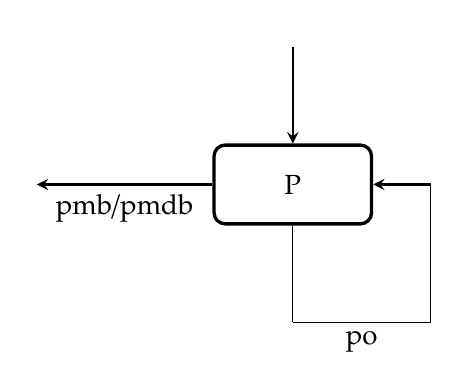
\begin{tikzpicture}[node distance=1.75cm]
    \tikzstyle{in_out} = [rectangle, rounded corners, minimum width=2cm, minimum height=1cm, text centered, draw=black, very thick]%, fill=red!30]
    \tikzstyle{rect} = [rectangle, rounded corners, minimum width=3cm, minimum height=1cm, text centered, draw=black]
    \tikzstyle{process} = [rectangle, rounded corners, minimum width=0.75cm, minimum height=0.75cm,text centered, draw=black, fill=gray!12.5]
    \tikzstyle{intersection} = [rectangle, rounded corners, minimum width=4cm, minimum height=1cm, text centered, draw=black]
    \tikzstyle{arrow} = [thick,->,>=stealth]

    \node (InputP) [in_out, xshift=0cm] {P};

    \node (InvIn) [coordinate, above of=InputP, xshift=0cm, yshift=-0cm, label=] {};
    \node (InvOut) [coordinate, left of=InputP, xshift=-1.5cm, yshift=-0cm, label=] {};

    \node (Inv1) [coordinate, below of=InputP, xshift=0cm, yshift=-0cm, label=] {};
    \node (Inv2) [coordinate, right of=Inv1, xshift=0cm, yshift=-0cm, label=] {};
    \node (Inv3) [coordinate, above of=Inv2, xshift=0cm, yshift=-0cm, label=] {};

    % ----- ----- ----- ----- ----- ----- ----- ----- ----- ----- ----- ----- ----- ----- ----- ----- ----- ----- -----

    \draw [arrow] (InvIn) -- node[anchor=east] {} (InputP);

    \draw (InputP) -- node[anchor=east] {} (Inv1);
    \draw (Inv1) -- node[anchor=north] {po} (Inv2);
    \draw (Inv2) -- node[anchor=east] {} (Inv3);
    \draw [arrow] (Inv3) -- node[anchor=east] {} (InputP);

    \draw [arrow] (InputP) -- node[anchor=north] {pmb/pmdb} (InvOut);
\end{tikzpicture}
\caption{$P$ can produce itself. $pmd$ should only created, when at least one time $P$ created itself.}
\label{fig:OldStyleMultiplePositions}
\end{figure}

$P$ can create correct words. But it cannot determine, whether at least one time $P$ created itself. So all words \dashAndSpaceSeq{with and without} summary prefix can be created. In a programming language we could use a flag or something similar to distinguish this two cases. In a CFG this approach is not usable, because we don't have variables or other kind of states, that can be altered. The only possibility to solve this issue is to introduce a new \nonterminal\space \dashAndSpace here called $P_2$. For the sake of completeness we rename $P$ to $P_1$.\\

$P_2$ can only be reached, if at least one times $po$ was produced. So the usage of the \nonterminal\space $P_2$ itself holds the information, that a summary prefix must be used. Figure \ref{fig:NewStyleMultiplePositions} shows the modified visualization of $P$.

\begin{figure}[H]
\centering
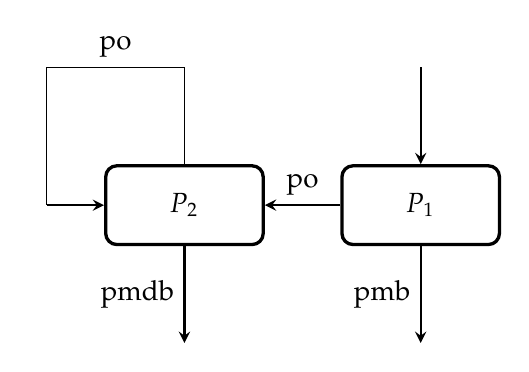
\begin{tikzpicture}[node distance=1.75cm]
    \tikzstyle{in_out} = [rectangle, rounded corners, minimum width=2cm, minimum height=1cm, text centered, draw=black, very thick]%, fill=red!30]
    \tikzstyle{rect} = [rectangle, rounded corners, minimum width=3cm, minimum height=1cm, text centered, draw=black]
    \tikzstyle{process} = [rectangle, rounded corners, minimum width=0.75cm, minimum height=0.75cm,text centered, draw=black, fill=gray!12.5]
    \tikzstyle{intersection} = [rectangle, rounded corners, minimum width=4cm, minimum height=1cm, text centered, draw=black]
    \tikzstyle{arrow} = [thick,->,>=stealth]

    \node (InputP1) [in_out, xshift=0cm] {$P_1$};
    \node (InputP2) [in_out, xshift=-3cm] {$P_2$};

    \node (InvIn) [coordinate, above of=InputP1, xshift=0cm, yshift=-0cm, label=] {};
    \node (InvOut2) [coordinate, below of=InputP2, xshift=0cm, yshift=-0cm, label=] {};
    \node (InvOut1) [coordinate, below of=InputP1, xshift=0cm, yshift=-0cm, label=] {};

    \node (Inv1) [coordinate, above of=InputP2, xshift=0cm, yshift=-0cm, label=] {};
    \node (Inv2) [coordinate, left of=Inv1, xshift=0cm, yshift=-0cm, label=] {};
    \node (Inv3) [coordinate, below of=Inv2, xshift=0cm, yshift=-0cm, label=] {};

    % ----- ----- ----- ----- ----- ----- ----- ----- ----- ----- ----- ----- ----- ----- ----- ----- ----- ----- -----

    \draw [arrow] (InvIn) -- node[anchor=east] {} (InputP1);
    \draw [arrow] (InputP1) -- node[anchor=east] {pmb} (InvOut1);

    % P1 -> P2
    \draw [arrow] (InputP1) -- node[anchor=south] {po} (InputP2);

    \draw (InputP2) -- node[anchor=east] {} (Inv1);
    \draw (Inv1) -- node[anchor=south] {po} (Inv2);
    \draw (Inv2) -- node[anchor=east] {} (Inv3);
    \draw [arrow] (Inv3) -- node[anchor=east] {} (InputP2);
    \draw [arrow] (InputP2) -- node[anchor=east] {pmdb} (InvOut2);
\end{tikzpicture}
\caption{Modified $P$. The usage of $P_2$ gurantees, that at least one times $po$ was created.}
\label{fig:NewStyleMultiplePositions}
\end{figure}

\begin{figure}[H]
    \begin{minipage}[l]{\CFGDefinitionSize\textwidth}
        $$
        \begin{aligned}
            T &=& \{c, p, m, b, o, d\} \\
            N &=& \{S, M, {\color{\colorNew}P_1, P_2}\} \\
            P &:& \\
            S &\rightarrow& M \\
            M &\rightarrow& {\color{\colorNew}P_1}c \\
            M &\rightarrow& c \\
            % {\color{\colorNew}M} &\rightarrow& {\color{\colorNew}C} \\
            {\color{\colorNew}P_1} &\rightarrow& {\color{\colorNew}pmb} \\
            {\color{\colorNew}P_1} &\rightarrow& {\color{\colorNew}poP_2} \\
            {\color{\colorNew}P_2} &\rightarrow& {\color{\colorNew}poP_2} \\
            {\color{\colorNew}P_2} &\rightarrow& {\color{\colorNew}pmdb} \\
        \end{aligned}
        $$
        \caption{Adjusted CFG with $P_1$ and $P_2$.}
        \label{fig:CFGWithMultipleBranchesAtTheSameLengthNewApproach}
    \end{minipage}
    \begin{minipage}[r]{\SymbolDescriptionTable\textwidth}
        \begin{table}[H]
        \centering
            \begin{tabular}{c|l}
                \toprule
                \textbf{Symbol} & \textbf{Description} \\
                \midrule
                c & Main chain \\
                p & position \\
                m & minus char \\
                b & branch \\
                o & comma char \\
                d & summary prefix \\
                \bottomrule
            \end{tabular}
            %\captionVSpace
            %\caption{Descriptions of the terminal symbols}
        \end{table}
    \end{minipage}
\end{figure}

We see, that our grammar uses now complete new production rules. One noticeable change are the production rules $P_1$ and $P_2$ with the same result $poP_2$. This is an usual way to define loops in a CFG. With the altered CFG, the production of the valid word \emph{2,3-DiMethylHeptan} is also modified:
$
S
{\color{\colorBracketFirstNesting}{(}}
    M
    {\color{\colorBracketSecondNesting}{(}}
        P_1
        {\color{\colorBracketThirdNesting}{(}}
            po,
            P_2
            {\color{\colorBracketFourthNesting}{(}}
                pmdb
            {\color{\colorBracketFourthNesting}{)}}
        {\color{\colorBracketThirdNesting}{)}}
        , c
    {\color{\colorBracketSecondNesting}{)}}
{\color{\colorBracketFirstNesting}{)}}
$.



\section{Second order branches}\label{ss:SecondOrderBranches}
In the chapter \ref{ss:FirstOrderBranches} and \ref{ss:MultipleFirstOrderBranches} first order branches are used. There are also so called \gerquot{second order branches}. This is are nested branch, that is connected to a first order branch. Maybe the question can occur, how many nesting steps are possible. The nomenclature itself defines no limit\footnote{In normal cases chemicals with a deeper nesting than second order branches are not stable. So the real life gives a practical limit.}. Figure \ref{fig:FourthExample} is an easy example for a second order branch.

\begin{figure}[H]
    \centering
    \setchemfig{chemfig style={line width=\connectionThicknessDefault}}
    \chemfig{C-[,,,,\colorMainChain]C-[,,,,\colorMainChain]C-[,,,,\colorMainChain]C
    (-[6,,,,\colorBranchFirstNesting]C(-[0,,,,\colorBranchSecondNesting]C)-[6,,,,\colorBranchFirstNesting]C)
    -[,,,,\colorMainChain]C-[,,,,\colorMainChain]C-[,,,,\colorMainChain]C} \\
    \caption{Example of a second order branch. The cyan connection is the second order branch.}
    \label{fig:FourthExample}
\end{figure}

The last chapters explained how to handle a first order branch. Here: It has a length of two carbon atoms ($\rightarrow$ \emph{Ethyl}) on the fourth position $\rightarrow$ \emph{4-Ethyl}. The IUPAC nomenclature handles a nesting with encapsulation of these in parentheses. The position of the nested branch is determined by the connection to the branch with the upper order (here \emph{1}). And the length is described with the common rule for branches. The position of the upper order branch will be written before the opening parentheses to make clear on which upper branch the nesting is connected to. The solution for the branch in our example makes it more understandable: \emph{4-(1-Methyl)EthylHeptan}.

In words: On a main chain with the length 7 \dashAndSpace there is a first order branch at the fourth position with the length 2. And on this branch is on the first position a nested branch with the length 1.

The current CFG is not designed to describe nestings. An adjustment would be necessary. The example with nested branches shows, that already described elements are only a tiny part of the whole nomenclature. However for this project it sufficient.

% The current CFG is not designed to describe nestings. So we need to alter it. At the begin two new terminal symbols for the parentheses: $x$ for the \texttt{\textbf{(}} and $y$ for \texttt{\textbf{)}}. The part with the most difficulties is the number of nestings. We need to close every parentheses and we are not allowed to have more closing parentheses than opening. An usual way to achieve this is a \nonterminal\space, that creates the opening and the closing symbol \dashAndSpace without any intermediate steps. E.g.: A{\color{red}{x}}B{\color{red}{y}}C With this rule there are always the same number of opening and closing parentheses.\\





% Aus Zeitgruenden und weil laut Thorsten dieser Bericht eher eine Formalie sei, wuerde ich mir nicht mehr die Arbeit machen und einen konkreten Syntaxbaum fuer ein Beispiel zu erstellen.
%\section{Abstract- and Concrete Syntax Trees}\label{s:AbstractAndConcreteSyntaxTrees}
\section{Abstract syntax tree: An example}\label{s:AbstractSyntaxTreeAnExample}
In the section \ref{s:IntroductionToTheIUPACNomenclature} we used the tuple description of the CFG. Now we show here an example of an abstract syntax tree to simplify the visualization of a parsing process and focusing on structural details instead of describing the whole language with every intermediate step.
% In this description type every detail of the language is defined. And the production even of a simple word contains multiple nested parentheses. Also to mention is the missing possibility to give the Terminal- and Non-Terminalsymbols more expressive names instead of exact one char.\footnote{The tuple description is a mathematical way to describe a grammar.} Already with a few production rules, the grammar becomes complex to handle and especially to debug (see chapter \ref{ss:MultipleFirstOrderBranches}).

% For this reason the syntax tree was invented. This is a more graphical way to describe a production rule of a word in a specific grammar. The abstract syntax tree focuses on the structural details instead of describing the whole language with every intermediate step in a formal manner. The CFG from figure \ref{fig:CFGWithMultipleBranchesAtTheSameLengthNewApproach} with the \emph{2,3-DiMethylHeptan} could be represented shown in figure \ref{fig:AbstractSyntaxTreeFirstExample}.

In figure \ref{fig:AbstractSyntaxTreeExample} the main structure of the production  is immediately noticeable. For example, that \gerquot{Position 2 with length} creates the position, the summary prefix \emph{and} the branch. This is not an error \dashAndSpace it is here a design choice.

\newcommand{\colorASTNode}{blue!15}
\newcommand{\colorASTNodeAtTheEnd}{green!40}
\begin{figure}[H]
\centering
% Main structure code from: https://texample.net/tikz/examples/tree/
\begin{tikzpicture}
    [sibling distance=16em,
    every node/.style = {shape=rectangle,
    % draw,
    align=center,
    top color=\colorASTNode, bottom color=\colorASTNode}]
    \node {IUPAC name}
    child { node {First order branch}
        child { node {Position 1}
            child { node[top color=\colorASTNodeAtTheEnd, bottom color=\colorASTNodeAtTheEnd] {\textbf{2,}} } }
        child { node {Position 2 with length}
            child { node[top color=\colorASTNodeAtTheEnd, bottom color=\colorASTNodeAtTheEnd] {\textbf{3-DiMethyl}} } } }
    child { node {Main chain}
        child { node[top color=\colorASTNodeAtTheEnd, bottom color=\colorASTNodeAtTheEnd] {\textbf{Heptan}} } };
\end{tikzpicture}
\caption{Abstract syntax tree of the word \emph{2,3-DiMethylHeptan}.}
\label{fig:AbstractSyntaxTreeExample}
\end{figure}


\chapter{Xtext}\label{s:Xtext}
In this section, we show how the domain was implemented as a \metamodel\space and the resulting Xtext code. We also show examples from section \ref{s:IntroductionToTheIUPACNomenclature} in the generated editor, where our domain-specific language is used.  

\section{Abstract Syntax: Meta Model}\label{ss:AbstractSyntax:Metamodel}
With \metamodel ing we model the abstract syntax of our DSL. We here designed our \metamodel \space (Figure \ref{fig:SSIUPACMetaModel}) with the modeling language \emph{Ecore} from the \emph{Eclipse Modelling Framework (EMF)}. How to create such a \metamodel\space is described here\footnote{Appendix B: Eclipse Modeling Framework}. Now, we want to look at the classes and how they're connected. We're also particularly interested in their attributes, especially these from type Enum. 

%%%%% BEGIN Meta Model Screenshot %%%%%
\begin{figure}[H]
\centering
\includegraphics[width=0.99\textwidth]{./Screenshots/Meta_Modell_With_Nesting.png}
\caption{Meta model of the IUPAC nomenclature.}
\label{fig:SSIUPACMetaModel}
\end{figure}
%%%%% END Meta Model Screenshot %%%%%

The \emph{IUPAC} class serves as the \metamodel\space class, and each of the other classes (\emph{Chain, Branch, SummaryPrefix, Position}) is a component of this class. This relationship is realized through a \emph{composition} with a cardinality of \emph{0 to many}. Through these relationships, we aim to convey that numerous nomenclatures can be created.

We started describing in section \ref{ss:NothingThanStraightChains}, that the IUPAC nomenclature must have at least a main chain. In the class diagram, we assigned a different name to it. This decision was made, because we omit the semantic rules between the main chain and branch. We have chosen an Enum to store the \emph{encoded names} of our \emph{Chain class} \dashAndSpace just like described in table \ref{tab:NumCarbonEncodedName}.
With this Enum, we have also established a framework for specifying the number of carbon atoms in a straight line that we intend to encode. Our goal is to encode a maximum of ten carbon atoms in a straight line without any branches. Now that we have established the foundation with the \emph{Chain class}, the remaining classes are derived hierarchically from it.

Through the composition relationship from the \emph{Chain class}, we constrained the \emph{encoding of chains} to those having a maximum of two branches aligned. These branches are defined as \emph{encoded branch names} and are also stored in an Enum. \\

Without any branches, we can not derive the prefix and the position information. That's why the two classes \emph{SummaryPrefix} and \emph{Position} are part of the \emph{Branch class} via a composition. From Figure \ref{fig:CFGWithMultipleBranchesAtTheSameLengthNewApproach}, we can derive, that there must be in total one prefix, when position information are introduced.

Alternatively, when defining a prefix based on this, you must specify the exact number of distinct position information. In the meta-model, the \emph{1 to 4 relationship} indicates that up to four position information can be utilized in an IUPAC name, resulting in an Enum of up to four distinct prefixes. Initially, the number four may seem arbitrary, yet it aids in minimizing the verbosity of our domain-specific language. 

Our position information is stored in an Enum, limited to ten different position names. This constraint aligns with our specification that the main chain can contain up to ten carbon atoms. 

Since the syntax of Ecore requires to define default values, we have decided to take the IUPAC name from Figure \ref{fig:SecondExample}. Last but not least, let's take a look at nesting, which was realised using the \emph{Branch class}. This implements what appears in section \ref{ss:SecondOrderBranches} Here, however, we again restrict the fact that only one branch can be nested in a branch. For the time being, we assume that you can nest an infinite number of times. \\


\section{Static Semantic: OCL Constraints}\label{ss:StaticSemantic:OCLConstraints}

In section \ref{ss:MultipleFirstOrderBranches} static semantic was briefly touched upon.There are more static semantic rules describing how the IUPAC name should look like. To add those rules we used the textual editor of Ecore. There we implemented so-called OCL constraints to define the static semantics of our DSL. However, we have implemented three OCL constraints in total. This was initially sufficient for our project.  

We considered the following semantic rules:  

\begin{enumerate}
    \item The number of position information must be compatible with the prefix.
    \item If there are more than one position information, then these must be in ascending order.
    \item If there are several branches, they must be sorted alphabetically. 
\end{enumerate} 

\section{Concrete Syntax: Xtext Code}\label{ss:ConcreteSyntax:Xtextcode}
 
\begin{lstlisting}[language=Xtext, numbers=none]
// Our adjusted Xtext code
grammar org.xtext.example.mydsl.MyDsl

import "http://IUPAC.ecore" 
import "http://www.eclipse.org/emf/2002/Ecore" as ecore

IUPAC returns IUPAC:
//IUPAC class is mandatory to Object instantiation of EOL or 
//Chain.   
	{IUPAC} 
	EOL*
	((chain+=Chain)EOL+)*;
	
Chain returns Chain:
//Chain class is mandatory, to derive a correct IUPAC name.
	{Chain} 
		((branch+=Branch) ("-" branch+=Branch)*)? 
  //Provide more branches with different lengths 
 		encodedName=EncodedName;
		
enum EncodedName returns EncodedName:
	Methan = "Methan" | Ethan = "Ethan" | 
    Propan = "Propan" | Butan = "Butan" | 
    Pentan = "Pentan" | Hexan = "Hexan" | 
	Heptan = "Heptan" | Octan = "Octan" | 
    Nonan = "Nonan" | Decan = "Decan";

Branch returns Branch:
	(position +=Position ("," position += Position)*) "-" 
	("("branch=Branch")")? //Nested branches       
	summaryprefix=SummaryPrefix
	branchName=EncodedBranchName;
\end{lstlisting}
\begin{lstlisting}[language=Xtext, numbers=none]
enum EncodedBranchName returns EncodedBranchName:
	Methyl = "Methyl" | Ethyl = "Ethyl" | 
    Propyl = "Propyl" | Butyl = "Butyl";

SummaryPrefix returns SummaryPrefix:
	prefix=Prefix;

Position returns Position:
	digit=PositionInformation;

enum Prefix returns Prefix:
	Mono = "Mono" | Di = "Di" | Tri = "Tri" | Tetra = "Tetra";
\end{lstlisting}
\begin{figure}[H]
\centering
\begin{lstlisting}[language=Xtext, numbers=none]
enum PositionInformation returns PositionInformation:
	One = "1" | Two = "2" | Three = "3" | Four = "4" | 
	Five = "5" | Six = "6" | Seven = "7" | 
	Eight = "8" | Nine = "9" | Ten = "10";
 
//EOL means end of line. 
//Here we realize that every IUPAC name is completed,
//when a new line begins or a comment is attached 
//at the end of the IUPAC name. 
EOL:
	NEWLINE | SL_COMMENT;

terminal SL_COMMENT:
	"//" !("\n"|"\r")* ("\r"? "\n")?;
	
terminal NEWLINE:
	("\r"? "\n");

\end{lstlisting}
\caption{Our concrete syntax definition adjusted, after deriving from the IUPAC meta-model.}
\label{fig:XtextCode}
\end{figure}

After implementing the meta-model and OCL constraints, our attention turned to refining the syntax. We utilized our meta-model to generate Xtext code, which we further customized. The syntax of the Xtext code is inspired from the \ENBF (EBNF). For instance, we encoded position information as numerical values and adjusted the order of IUPAC names.

Each class from our meta-model finds representation in our Xtext code. The red-highlighted elements in Figure \ref{fig:XtextCode} denote our literals, reflecting the language's vocabulary. These literals are entered within the generated editor as you will see in section \ref{ss:DSLEditor}. The previously defined composition relation ensures a specific order for entering the literals. Introducing special characters such as \textcolor{red}{","}, or \textcolor{red}{"-"}, provide a more concrete representation of our domain. The cardinalities from the relations are represented in Xtext with symbols such as " \textcolor{green}{=}, \textcolor{green}{*}, or \textcolor{green}{+=} ". \\

We also needed to introduce \emph{EOL} as \nonterminal\space to reduce to terminal symbols. These are on the one hand the comment symbol \textcolor{red}{"//"} and on the other hand the newline symbols (\textcolor{red}{"\textbackslash r"} or \textcolor{red}{"\textbackslash n"}), which are indicating an empty word ($\epsilon$). This separates the IUPAC names from each other in the editor, because We did not classify the literals of the IUPAC name as terminals. The comment symbol allows us to comment our code.\\

Like in \CFG\space, we can also replace in our Xtext code \nonterminal s, with other \nonterminal s, multiple \nonterminal s or \nonterminal s with literal symbols. In Figure \ref{fig:CFGinXtext} we have shown schematically how our Xtext code would look in \CFG\space and then we show how to derive a specific IUPAC name from it.\\

\lstset{
  basicstyle=\itshape,
  xleftmargin=3em,
  literate={->}{$\rightarrow$}{2}
           {ϵ}{$\epsilon$}{1}
           {δ}{$\delta$}{1}
}

\begin{figure}[H]
\noindent Classes:\\ 
\texttt{\phantom{XXXX}S\multido{}{21}{\space}$\rightarrow$\space IUPAC | EOL}\\
\texttt{\phantom{XXXX}IUPAC\multido{}{17}{\space}$\rightarrow$\space ChainEOL}\\
\texttt{\phantom{XXXX}Chain\multido{}{17}{\space}$\rightarrow$\space BranchEncodedName | EncodedName}\\
\texttt{\phantom{XXXX}Branch\multido{}{16}{\space}$\rightarrow$\space Branch-Branch}\\
\texttt{\phantom{XXXX}Branch\multido{}{16}{\space}$\rightarrow$\space Position-SummaryPrefixEncodedBranchName |} 
\texttt{\phantom{xxxxxxxxxxxxxxxxxxxxxxxxxxxxx}Position-(Branch)SummaryPrefixEncodedBranchName}\\
\texttt{\phantom{XXXX}Position\multido{}{14}{\space}$\rightarrow$\space Position,Position}\\
\texttt{\phantom{XXXX}Position\multido{}{14}{\space}$\rightarrow$\space PositionInformation}\\
\texttt{\phantom{XXXX}SummaryPrefix\multido{}{9}{\space}$\rightarrow$\space Prefix}\\

%\begin{lstlisting}
%IUPAC         -> ChainEOL
%Chain         -> BranchEncodedName | EncodedName
%Branch        -> Branch-Branch
%Branch        -> Position-SummaryPrefixEncodedBranchName | 
%                 Position-(Branch)SummaryPrefixEncodedBranchName
%Position      -> Position, Position
%Position      -> PositionInformation 
%SummaryPrefix -> Prefix
%\end{lstlisting}

\noindent Enumerations:\\
\texttt{\phantom{XXXX}EncodedName\multido{}{11}{\space}$\rightarrow$\space Methan | Ethan | ...}\\
\texttt{\phantom{XXXX}EncodedBranchName\multido{}{5}{\space}$\rightarrow$\space Methyl | Ethyl | ...}\\
\texttt{\phantom{XXXX}PositionInformation\multido{}{3}{\space}$\rightarrow$\space 1 | 2 | 3 | ...}\\
\texttt{\phantom{XXXX}Prefix\multido{}{16}{\space}$\rightarrow$\space Mono | Di | Tri | ...}\\

%\begin{lstlisting}
%EncodedName         -> Methan | Ethan | ...
%EncodedBranchName   -> Methyl | Ethyl | ...
%PositionInformation -> 1 | 2 | 3 | ...
%Prefix              -> Mono | Di | Tri | ...
%\end{lstlisting}

\noindent End of line:\\
\texttt{\phantom{XXXX}EOL\multido{}{19}{\space}$\rightarrow$\space // | 
$\epsilon$}
%\begin{lstlisting}
%EOL                 -> // | ϵ 
%\end{lstlisting}
    \caption{Our Xtext code in \CFG \space form. \emph{S} is here the start symbol. A IUPAC name can be terminated with either \emph{//} or $\epsilon$.}
    \label{fig:CFGinXtext}
\end{figure}

\begin{figure}[H]
    \noindent Example:\\
    \texttt{\phantom{XXXX}S\multido{}{4}{\space}$\rightarrow$\space IUPAC}\\
    \texttt{\phantom{X}\multido{}{8}{\space}$\rightarrow$\space ChainEOL}\\
    \texttt{\phantom{X}\multido{}{8}{\space}$\rightarrow$\space Chain}\\
    \texttt{\phantom{X}\multido{}{8}{\space}$\rightarrow$\space BranchEncodedName}\\ 
    \texttt{\phantom{X}\multido{}{8}{\space}$\rightarrow$\space BranchHeptan}\\
    \texttt{\phantom{X}\multido{}{8}{\space}$\rightarrow$\space Position-SummaryPrefixEncodedBranchNameHeptan}\\
    \texttt{\phantom{X}\multido{}{8}{\space}$\rightarrow$\space Position,Position-SummaryPrefixEncodedBranchNameHeptan}\\
    \texttt{\phantom{X}\multido{}{8}{\space}$\rightarrow$\space Positioninformation,Positioninformation-PrefixMethylHeptan}\\
    \texttt{\phantom{X}\multido{}{8}{\space}$\rightarrow$\space 2,3-DiMethylHeptan}\\
% \begin{lstlisting}
% S -> IUPAC 
% -> ChainEOL 
% -> Chain 
% -> BranchEncodedName 
% -> BranchHeptan 
% -> Position-SummaryPrefixEncodedBranchNameHeptan 
% -> Position,Position-SummaryPrefixEncodedBranchNameHeptan
% -> Positioninformation,Positioninformation-PrefixMethylHeptan
% -> 2,3-DiMethylHeptan
% \end{lstlisting}
    \caption{From our "Xtext" grammar, we can derive this IUPAC name.}
    \label{fig:ExampleWordFromCFG}
\end{figure}

\section{DSL: Editor}\label{ss:DSLEditor}

%%%%% BEGIN Editor Screenshot %%%%%
\begin{figure}[H]
    \centering
    \includegraphics[width=\screenshotWidth\textwidth]{./Screenshots/GraphicalEditor.PNG}
    \caption{Generated editor with static semantics of \ref{ss:StaticSemantic:OCLConstraints} and default concrete syntax of \ref{ss:ConcreteSyntax:Xtextcode}. It also highlights the negative example and outputs the concrete error.}
    \label{fig:GraphicalEditor}
\end{figure}
%%%%% END Editor Screenshot %%%%%

The generated Editor can do syntax highlighting, performs static validation and code completion, when you type. Figure \ref{fig:GraphicalEditor} shows the Editor, which accepts the IUPAC names from our previous sections. It also detects the mistake from the last IUPAC name, where prefix and branch name are swapped.

\section{Possible use cases}\label{ss:PossibleUseCases}
One obvious use case is the validation of given IUPAC names. In figure \ref{fig:GraphicalEditor} is shown, that the generated editor indicates wrong names. Another idea could be an extended grammar with a grouping function. E.g.: The grammar accepts only names with a specific chain length. 



\chapter{Discussion and Conclusion}\label{s:DiscussionandConclusion}
Although it is possible to generate corresponding Xtext code for the \metamodel\space shown in \ref{fig:SSIUPACMetaModel}, such crude code is barely maintainable and expandable. Because we always need to update our meta model first. Otherwise newly added variables and data structures are unknown.\\

The generated Xtext code out of the Ecore model needed to be highly customized due the fact, that by default all terminals are handled as individual tokens without direct concatenation. In the original code the valid name \emph{2-MonoMethylHeptan} was only valid as such: \emph{2-Mono\textvisiblespace Methyl\textvisiblespace Heptan}.

Also the typical problem with results from parser generators and few meaningful error messages occurs here. In figure \ref{fig:GraphicalEditor} the word \emph{2,3,4-MethylTriHeptan} is wrong\footnote{The correct name is: \emph{2,3,4-TriMethylHeptan}} because \emph{Methyl} needs to be swapped with \emph{Tri}. The given error messages \gerquot{no viable alternative at input 'Methyl'} and \gerquot{no viable alternative at input 'Tri'} are hardly usable, especially for novice and intermediate users of such a DSL. A more meaningful message could be here: \gerquot{Missing summary prefix after list of positions.}.\\

In summary we made the experience with Ecore, that this technology is suitable for prototype- and test-DSLs. The generated Xtext code is not usable for productive use-cases due to a lot of adaptation work may be necessary. The fact that the code has to be completely rewritten if the model is changed reinforces our opinion that Ecore is hardly suitable for practical use. The generated Xtext code can at most be used as the basis for a DSL. On its own, Xtext is a fairly straightforward language for DSLs and is more useful for daily usage. Although the problem with the less expressive error messages is basically not solvable; it can be compensated by additional error production rules.



\chapter{Reflection}\label{s:Reflection}
In this section the reflection questions will be answered. The following question list was given:\footnote{Source of the questions: \href{https://moodle.ruhr-uni-bochum.de/pluginfile.php/1902788/mod_page/content/5/Reflexion.pdf}{\url{https://moodle.ruhr-uni-bochum.de/pluginfile.php/1902788/mod_page/content/5/Reflexion.pdf}}}

\begin{enumerate}
    \item Has the task or your understanding of the task changed over time? If so, how?
    \item How appropriate was the planning of the project, especially the intermediate-deadlines? How often did the planning have to be adjusted? Why? What was your role in this?
    \item What methods did you use to support the project planning and how did they work?
    \item How did the coordination of the project work? What problems were there? How were they solved? What was your role in this?
    \item To what extent were you sufficiently competent to cooperate? Which skills did you have to acquire in the course of the project? What did you learn learned from the study project?
    \item What have you done to work as efficiently and reliably as possible in the project?
    \item What would you do differently if you had to work on the task again with the experience at the end of the project?
    \item What challenges came in terms of group dynamics in the team and how did you deal with them?
\end{enumerate}

\section{Answered questions: Dominik Habermann}\label{ss:AnsweredQuestionsDominikHabermann}
\begin{enumerate}
    \item The main task was in the whole project the same. However some details were changed over time. For example: Topics that should be explained in the tutorial were added and/or altered.
    \item The intermediate-deadlines were changed multiple times. One major problem was to find dates for the meetings. The reason was, that there were only few time slots on which everyone was available. My part of this situation was the long drive home. Due to the lack of stable mobile internet, it was not possible to join a meeting.
    \item My method to support the project planning was to reserve exclusively fixed points of time in a week.
    \item See answer 2 and 3: The main problem was finding a time to meet together. My part of problems in the coordination was, that I don't like to be available the whole time. Usually I mute my phone when I at home.
    \item I was able to contribute my knowledge right from the start. I had to learn how to use the program called Eclipse and the Xtext framework; I hadn't worked much with this program until the project started. And the Xtext framework was completely unknown to me up to that point.
    \item I gave my team member tutorials and examples of the background topic. Because of private projects, the topic was not new to me. For reliably I installed on my machine an instant messaging client, which I don't used before on this device, and put them to the auto-start list. See answer of question 4.
    \item With the experience at the end of the project I would use a different way to finding times for meetings. For example, a more flexible selection of time periods would have helped right from the start.
    \item Not too much can be said about the challenges in group dynamics. In summary, there were no real problems regard to this.
\end{enumerate}

\section{Answered questions: Masuthan Mathiyalakan}\label{ss:AnsweredQuestionsMasuthanMathiyalakan}
\begin{enumerate}
    \item The requirements themselves have not changed. However, it was not entirely clear at the beginning in which direction the domain should go. There were also adjustments to the definition of the domain, to what extent we wanted to describe it in detail. Here and there, tasks were also adjusted, depending on the time frame.    
    \item The planning itself was sometimes not clearly structured. Both of us had regular meetings with our supervisor as well as regular group meetings in our core group, but sometimes, due to conflicts with other appointments, we had to cancel our meetings. Most of the time, we could rely on the appointments set by the supervisor. Occasionally, when one of us couldn't attend, the other person conducted the meeting with the supervisor or suggested an alternative appointment when they were unavailable. 
    \item The communication took place via email. Meetings were held regularly via Zoom. We usually suggested times to each other and when we reached a consensus, we entered the meeting in the calendar.  
    \item Dominik Habermann had suggested the IUPAC nomenclature domain. Consequently, he focused more on the definition of the domain itself. Since we were supposed to develop a DSL in Xtext, I concentrated on the creation of the \metamodel as well as the generation of Xtext code. Because the Xtext code has to be adapted to the domain, Dominik also helped me a lot in this case. The coordination was therefore fluent. We presented every week to each other, what we have done. If anyone had any further questions, someone answered as fast as possible. We had sometimes the problem to find a good date for a meeting with our supervisor. Thus we managed to send our status quo via mail.   
    \item As I am new to the DSL and IUPAC nomenclature field, I had to familiarize myself with these topics. I incorporated my experience from software development into the project. In addition to understanding the domain itself and creating DSLs using Xtext, I also gained knowledge on how to describe a domain in classes and create a metamodel. I also grasped the close integration of context-free grammar and IUPAC nomenclature.
    \item Always informed about the current status and as well as possible, the tasks for the next meetings. 
    \item Create a clear timetable from the outset as to when which milestone or goal must be completed. Schedule project meetings throughout the semester before the project starts. 
    \item There were no major problems, so there is nothing worth mentioning. 
\end{enumerate}

\end{document}
%%%%% %%%%% %%%%% %%%%% %%%%% %%%%% %%%%% %%%%%              %%%%% %%%%% %%%%% %%%%% %%%%% %%%%% %%%%% %%%%%
%%%%% %%%%% %%%%% %%%%% %%%%% %%%%% %%%%% %%%%% END document %%%%% %%%%% %%%%% %%%%% %%%%% %%%%% %%%%% %%%%%
%%%%% %%%%% %%%%% %%%%% %%%%% %%%%% %%%%% %%%%%              %%%%% %%%%% %%%%% %%%%% %%%%% %%%%% %%%%% %%%%%
